\chapter{Theory}

This work showcases the use of \glspl{pomdp} to model and solve decision making
problems in robotics with inherent uncertainty. In order to provide a baseline
for further discussions of specific application domains
(\cref{chap:applications}) we first introduce some of the throughout this work.
It should be noted that in the interest of conciseness we focus this
theoretical introduction on only the main tools use. Fundamental concepts of
statistical inference and tools like \textit{Monte Carlo Integration} are
assumed to be known. For a thorough discussion of these underlying concept the
reader may refer to \cite{kochenderfer2015decision} as well as
\cite{probRobotics}.\todo{Can I also assume knowledge of fully observable
MDPs?}

In the following, we first introduce the theoretical framework of \glspl{pomdp}
(\cref{sec:pomdp}). This section discusses modelling assumptions, structure
of solutions as well as theoretical properties of \glspl{pomdp}. Thereafter,
\cref{sec:online-pomdp-solvers} describes two state-of-the-art online solution
methods for problems of this domain.

\section{Partially Observable Markov Decision Processes}\label{sec:pomdp}

The \acf{pomdp} is a principled mathematical formalism capable of representing
a broad range of sequential decision making problems under uncertainty. As the
name suggests, this framework is a generalization of the more popular \ac{mdp}
to the partially observable case. Thus, before proceeding with the full
complexity of a \ac{pomdp} let us first examine it's fully observable version.

\subsection*{MDP}

\glspl{mdp} are sequential decision making problems in which an agent takes
\vname{actions} $a$ that affect the \vname{state} $s$ of the environment and
receives \vname{rewards} $r$ based the state-transition and the action taken
\cite{kochenderfer2015decision}. \todo{cite Bertsekas} The state evolves
according to a stochastic transition model $\mathcal{T}$ that and obeys the
Markov property. That is, \emph{future} states are \emph{independent} of
\emph{past} states given the current \vname{state} and \vname{action}. By this
means, \glspl{mdp} allow to model outcome uncertainty. As common in literature,
we denote quantities at time time $t$ with an according subscript. When examining
only a single step in a context where time does not explicitly matter, we may also
refer to the states before and after the transition as $s$ and $s'$ rather than
$s_t$ and $s_{t+1}$.

Formally, an \ac{mdp} is fully characterized by the following quantities:

\begin{description}
  \item[State Space $\mathcal{S}$.] The set of all possible states.
  \item[Action Space $\mathcal{A}$.] The set of all possible actions.
  \item[Transition Model $\mathcal{T}$.] A model to represent the likelihood of
    each transition. This model provides $\mathcal{T}(s' \mid s, a)$, the
    probability of state $s'$ given that previously the environment was in
    state $s$ and the agent took action $a$.
  \item[Reward Function $\mathcal{R}: \mathcal{S} \times \mathcal{A} \times
    \mathcal{S} \to \reals$.] A deterministic mapping that assigns
    a real-valued reward $r$ to each transition $(s, a, s')$ with finite transition
    probability, $\mathcal{T}(s' \mid s, a) > 0$.
  \item[Discount Factor $\gamma$.] A scalar that governs how \vname{rewards}
    are discounted in the future.
\end{description}

The objective of the agent in the \ac{mdp} is to maximize the expected
cumulative rewards. Formally, this translates to finding a \vname{policy} $\pi:
\mathcal{S} \to \mathcal{A}$, that maps each encountered $s$ to an action $a
= \pi(s)$, such that following this policy maximizes the objective,

\begin{equation} \label{eq:mdp-objective}
    J(\pi) = E\left[\sum_{t=0}^\infty \gamma^t \mathcal{R}(s_t, \pi(s_t), s_{t+1})\right] \text{.}
\end{equation}

An optimal solution to an \ac{mdp} can always be formulated as a deterministic
Markov policy, even though the reward that a policy achieves may be randomized
through $\mathcal{T}$. This is, there always exists a maximizer $\pi^*$ of
\cref{eq:mdp-objective}, where $\pi^*$ assign a single \vname{action} to every
\vname{state}. Also, since the state obeys the Markov property, no additional
information beyond the current state at every time is necessary to maximize $J$.

\subsection*{Partially Observable MDP}

The graphical representation of a \ac{pomdp}
as dynamic decision network is depicted in \cref{fig:pomdp}. \todo{Maybe change
order of things}.

\begin{figure}[htpb]
  \centering
  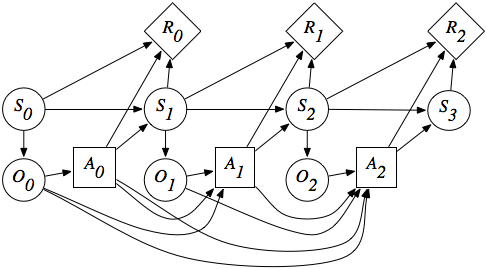
\includegraphics[width=.7\textwidth]{pomdp-dynamic-decision-network.png}
  \caption{The POMDP as a dynamic decision network. \todo[inline]{Replace with
  vector graphics.}}
  \label{fig:pomdp}
\end{figure}

\todo[inline]{brief definition of solutions to POMDPs as "conditional plans"
and point out that in general the full solution is intractable. Point to
complexity theory with some good source for this. (e.g. Mykel)}

\todo[inline]{Theoretical properties by modelling things in such a way. What
can be gained? What is the difference?}

\section{Online POMDP Solvers}\label{sec:online-pomdp-solvers}

\todo[inline]{The solvers described here were chosen as they are state of the
art and show good perfomance over a range of problems. Point to Zach's paper
for solver perfomance comparison and DESPOT paper.}

\section{POMCPOW}

\todo[inline]{write:}
\begin{itemize}
  \item explain the basic idea of POMCPOW as Monte Carlo with DPW.
  \item is extension of POMCP with weighted particle beliefs.
\end{itemize}
\missingfigure{Pseudo Code with formal description in text.}

\missingfigure{graphical model of POMCP-Tree with weighted scenarios.}

\section{DESPOT}

\todo[inline]{write:}
\begin{itemize}
  \item formal, high-level idea of a DESPOT (idea of scenarios etc.)
  \item the search algorithm on a DESPOT with bounds
  \item explain the difference to POMCPOW (or Monte Carlo methods in general)
  \item point to literature for convergence guarantees
\end{itemize}

\missingfigure{DESPOT tree visualization}
\missingfigure{DESPOT algorithm Pseudo Code}

